%===============================================================================
% LaTeX sjabloon voor de bachelorproef toegepaste informatica aan HOGENT
% Meer info op https://github.com/HoGentTIN/bachproef-latex-sjabloon
%===============================================================================

\documentclass{bachproef-tin}

\usepackage{hogent-thesis-titlepage} % Titelpagina conform aan HOGENT huisstijl
\usepackage[final]{pdfpages}
\usepackage{subcaption}
\usepackage{array}
\usepackage{pythonhighlight}

\newcolumntype{P}[1]{>{\centering\arraybackslash}p{#1}}
\newcolumntype{M}[1]{>{\centering\arraybackslash}m{#1}}

%%---------- Documenteigenschappen ---------------------------------------------
% TODO: Vul dit aan met je eigen info:

% De titel van het rapport/bachelorproef
\title{Classificatie van afbeeldingen met geautomatiseerde machine learning platformen}

% Je eigen naam
\author{Robbe Decorte}

% De naam van je promotor (lector van de opleiding)
\promotor{ir. Johan Decorte}

% De naam van je co-promotor. Als je promotor ook je opdrachtgever is en je
% dus ook inhoudelijk begeleidt (en enkel dan!), mag je dit leeg laten.
\copromotor{dr. Kenny Helsens}

% Indien je bachelorproef in opdracht van/in samenwerking met een bedrijf of
% externe organisatie geschreven is, geef je hier de naam. Zoniet laat je dit
% zoals het is.
\instelling{In The Pocket}

% Academiejaar
\academiejaar{2019-2020}

% Examenperiode
%  - 1e semester = 1e examenperiode => 1
%  - 2e semester = 2e examenperiode => 2
%  - tweede zit  = 3e examenperiode => 3
\examenperiode{2}

%===============================================================================
% Inhoud document
%===============================================================================

\begin{document}

%---------- Taalselectie -------------------------------------------------------
% Als je je bachelorproef in het Engels schrijft, haal dan onderstaande regel
% uit commentaar. Let op: de tekst op de voorkaft blijft in het Nederlands, en
% dat is ook de bedoeling!

%\selectlanguage{english}

%---------- Titelblad ----------------------------------------------------------
\inserttitlepage

%---------- Samenvatting, voorwoord --------------------------------------------
\usechapterimagefalse
%%=============================================================================
%% Voorwoord
%%=============================================================================

\chapter*{\IfLanguageName{dutch}{Woord vooraf}{Preface}}
\label{ch:voorwoord}

%% TODO:
%% Het voorwoord is het enige deel van de bachelorproef waar je vanuit je
%% eigen standpunt (``ik-vorm'') mag schrijven. Je kan hier bv. motiveren
%% waarom jij het onderwerp wil bespreken.
%% Vergeet ook niet te bedanken wie je geholpen/gesteund/... heeft


%%=============================================================================
%% Samenvatting
%%=============================================================================

% TODO: De "abstract" of samenvatting is een kernachtige (~ 1 blz. voor een
% thesis) synthese van het document.
%
% Deze aspecten moeten zeker aan bod komen:
% - Context: waarom is dit werk belangrijk?
% - Nood: waarom moest dit onderzocht worden?
% - Taak: wat heb je precies gedaan?
% - Object: wat staat in dit document geschreven?
% - Resultaat: wat was het resultaat?
% - Conclusie: wat is/zijn de belangrijkste conclusie(s)?
% - Perspectief: blijven er nog vragen open die in de toekomst nog kunnen
%    onderzocht worden? Wat is een mogelijk vervolg voor jouw onderzoek?
%
% LET OP! Een samenvatting is GEEN voorwoord!

%%---------- Nederlandse samenvatting -----------------------------------------
%
% TODO: Als je je bachelorproef in het Engels schrijft, moet je eerst een
% Nederlandse samenvatting invoegen. Haal daarvoor onderstaande code uit
% commentaar.
% Wie zijn bachelorproef in het Nederlands schrijft, kan dit negeren, de inhoud
% wordt niet in het document ingevoegd.

\IfLanguageName{english}{%
\selectlanguage{dutch}
\chapter*{Samenvatting}
\lipsum[1-4]
\selectlanguage{english}
}{}

%%---------- Samenvatting -----------------------------------------------------
% De samenvatting in de hoofdtaal van het document

\chapter*{\IfLanguageName{dutch}{Samenvatting}{Abstract}}

\lipsum[1-4]


%---------- Inhoudstafel -------------------------------------------------------
\pagestyle{empty} % Geen hoofding
\tableofcontents  % Voeg de inhoudstafel toe
\cleardoublepage  % Zorg dat volgende hoofstuk op een oneven pagina begint
\pagestyle{fancy} % Zet hoofding opnieuw aan

%---------- Lijst figuren, afkortingen, ... ------------------------------------

% Indien gewenst kan je hier een lijst van figuren/tabellen opgeven. Geef in
% dat geval je figuren/tabellen altijd een korte beschrijving:
%
%  \caption[korte beschrijving]{uitgebreide beschrijving}
%
% De korte beschrijving wordt gebruikt voor deze lijst, de uitgebreide staat bij
% de figuur of tabel zelf.

\listoffigures
\listoftables

% Als je een lijst van afkortingen of termen wil toevoegen, dan hoort die
% hier thuis. Gebruik bijvoorbeeld de ``glossaries'' package.
% https://www.overleaf.com/learn/latex/Glossaries

%---------- Kern ---------------------------------------------------------------

% De eerste hoofdstukken van een bachelorproef zijn meestal een inleiding op
% het onderwerp, literatuurstudie en verantwoording methodologie.
% Aarzel niet om een meer beschrijvende titel aan deze hoofstukken te geven of
% om bijvoorbeeld de inleiding en/of stand van zaken over meerdere hoofdstukken
% te verspreiden!

%%=============================================================================
%% Inleiding
%%=============================================================================

\chapter{\IfLanguageName{dutch}{Inleiding}{Introduction}}
\label{ch:inleiding}

Het informatie tijdperk centraliseert zich momenteel rond data. Bedrijven zien ook de toegevoegde waarde die het kan hebben in hun bedrijfsprocessen, kijk maar naar de grote spelers in de informaticawereld waar het begrip textit{Big Data} is ontstaan. In zijn ruwe vorm lijkt het op een gigantische hoop waaruit je niks kan leren, maar wanneer men deze gaat structureren zijn er plots allemaal nieuwe toepassingen beschikbaar. 
Eén van deze toepassingen die intensief gebruik maakt van data, is \textit{machine learning}. Hierbij wordt geprobeerd computers zaken aan te leren met behulp van een iteratief proces zonder expliciet geprogrammeerd te zijn voor de taken die ze uitvoeren. Mensen die goed overweg kunnen met de data om zo'n model te maken (Machine Learning Engineers / Data Scientists ...)  zijn vaak moeilijk te vinden. Een werkgever die zo'n probleem aan wilt pakken heeft enkele keuzes, AutoML is mogelijks een optie. Alhoewel het interesseveld ontstaan is in de jaren '50, is het nog maar sinds kort een hot topic met dank aan de grote hoeveelheid rekenkracht in moderne systemen en doorbraken\footnote{Denk maar aan \textit{open source} initiatieven zoals Tensorflow en Keras.} binnen het onderzoeksveld die de toegangsdrempel verlagen.

Geautomatiseerde \textit{machine learning} platformen trachten een oplossing te bieden voor \textit{development} teams zonder een gespecialiseerde \textit{machine learning} expert. Het platform voert alle stappen van het proces uit en uiteindelijk moeten ze het enkel in hun product integreren. Deze manier van werken verlaagt niet alleen de druk op \textit{machine learning} experten maar het geeft hen ook de mogelijkheid om mee te werken aan uitdagende projecten of zelf onderzoek te voeren. Door de technische afhankelijkheid te verlagen kan de technologie sneller / meer gebruikt worden in bestaande projecten. Omdat bedrijven tot nu toe weinig contact hebben met AI en alles wat er toe behoort, zijn de meeste cases vergelijkbaar met elkaar. Zo heb je bijvoorbeeld binaire classificatie problemen, tekst analyse en meer. Waarom zou het dan niet mogelijk zijn om dit te automatiseren? 

In dit onderzoek wordt bekeken hoe laag de werkelijke instapdrempel ligt bij verschillende platformen (open-source en private oplossingen), alsook hoe zo'n model werkt en welke resultaten je bekomt voor een simpel maar realistisch classificatie probleem.

\section{\IfLanguageName{dutch}{Probleemstelling}{Problem Statement}}
\label{sec:probleemstelling}

Met een onschatbare hoeveelheid data die de dag van vandaag aanwezig is, is het belangrijk om deze op te schonen en features te selecteren zodat het gebruikt kan worden in een specifieke situatie. De hoeveelheid data groeit vele malen sneller dan het aantal beschikbare experten. Er moet dus naar een manier gezocht worden om \textit{machine learning} dichter bij de man te brengen zodat mensen met een uitgebreide kennis niet vast zitten met basis problemen die ze eerder al op een gelijkaardige manier opgelost hebben. Er wordt over basisproblemen gesproken in de zin dat bedrijven een eigen toepassing willen op een probleem dat al vele malen opgelost is in andere situaties. Hierbij zijn de stappen van het trainingsproces in grote lijnen gelijk.

Het is dan ook vanzelfsprekend dat er gezocht wordt naar een manier om dit te automatiseren, zoals in elke ander aspect van ons leven. Deze platformen kunnen mogelijks een oplossing bieden voor kleine zelf organiserende \textit{development} teams die graag een \textit{machine learning} aspect willen toevoegen aan hun project. Dit liefst met een minimale input van de ontwikkelaars.

\section{\IfLanguageName{dutch}{Onderzoeksvraag}{Research question}}
\label{sec:onderzoeksvraag}

\subsection{Hoofdonderzoeksvraag}
\label{subsec:hoofdonderzoeksvraag}

Met dit onderzoek wordt nagegaan als deze nieuwe technologie capabel is om triviale machine learning problemen op te lossen, al dan niet met minimale input van een developer. Het is duidelijk dat AutoML in zijn huidige staat niet klaar is voor uitdagende cases, maar het kan wel toegang geven tot nieuwe functies aan \textit{development} teams met weinig of geen \textit{machine learning} kennis.

\subsection{Deelonderzoeksvragen}
\label{subsec:deelonderzoeksvragen}

Naast de hoofdonderzoeksvraag wordt er ook kort ingegaan en antwoord gegeven op:

\begin{itemize}
    \item Welke onderliggende technieken worden gebruikt bij geautomatiseerde machine learning.
    \item Kies je best voor een open source library of toch een commercieel platform.
    \item Is de performantie van deze platformen vergelijkbaar met die van een traditioneel gebouwd model.
\end{itemize}

\section{\IfLanguageName{dutch}{Onderzoeksdoelstelling}{Research objective}}
\label{sec:onderzoeksdoelstelling}

De belangrijkste doelstelling van dit onderzoek is reproduceren van een realistische situatie die op de traditionele manier opgelost is, maar dan met \textit{automated machine learning}. Dit is mogelijk door de verschillende metrieken en performaties van de modellen met elkaar te vergelijken. We zien het experiment als geslaagd als de behaalde scores bij elkaar in de buurt liggen. Een werkend prototype is de eerste stap.

Er zijn al verschillende mogelijkheden om dit te realiseren. Bij elke implementatie wordt dan ook getest hoeveel rekening er wordt gehouden met de belangrijkste aspecten\footnote{Aspecten die bepalen hoe bruikbaar de technologie is in de praktrijk} uit de \textit{requirements} analyse.

Aan de hand van de prototypes en de vergelijkende studie kan er een conclusie geschreven worden die rekening houdt met implementatie details en het standpunt van een bedrijf.

\section{\IfLanguageName{dutch}{Opzet van deze bachelorproef}{Structure of this bachelor thesis}}
\label{sec:opzet-bachelorproef}

% Het is gebruikelijk aan het einde van de inleiding een overzicht te
% geven van de opbouw van de rest van de tekst. Deze sectie bevat al een aanzet
% die je kan aanvullen/aanpassen in functie van je eigen tekst.

De rest van deze bachelorproef is als volgt opgebouwd:

In Hoofdstuk~\ref{ch:stand-van-zaken} wordt een overzicht gegeven van de stand van zaken binnen het onderzoeksdomein, op basis van een literatuurstudie.

In Hoofdstuk~\ref{ch:methodologie} wordt de methodologie toegelicht en worden de gebruikte onderzoekstechnieken besproken om een antwoord te kunnen formuleren op de onderzoeksvragen.

In Hoofdstuk~\ref{ch:autokeras} en \ref{ch:google-automl} wordt, respectievelijk, voor AutoKeras en Google Cloud AutoML een prototype opgezet en de \textit{requirements} besproken.

In Hoofdstuk~\ref{ch:conclusie}, tenslotte, wordt de conclusie gegeven en een antwoord geformuleerd op de onderzoeksvragen. Daarbij wordt ook een aanzet gegeven voor toekomstig onderzoek binnen dit domein.
\chapter{\IfLanguageName{dutch}{Stand van zaken}{State of the art}}
\label{ch:stand-van-zaken}

% Tip: Begin elk hoofdstuk met een paragraaf inleiding die beschrijft hoe
% dit hoofdstuk past binnen het geheel van de bachelorproef. Geef in het
% bijzonder aan wat de link is met het vorige en volgende hoofdstuk.

% Pas na deze inleidende paragraaf komt de eerste sectiehoofding.

Dit onderzoek richt zich op automatische machine learning platformen. Maar alvorens van start te gaan met de onderliggende technieken is het belangrijk om een goed zicht te hebben op de basis waarop het gebouwd is. Zo worden eerst een aantal belangrijke begrippen en technieken besproken, deze sectie kan overgeslagen worden als deze informatie triviaal is voor de lezer. De automatisatie hiervan wordt onderzocht, welke technieken worden met elkaar gecombineerd en hoe bekom je uiteindelijk resultaten. Het is nodig om de theoretische benadering goed te begrijpen om uiteindelijk te kunnen beslissen als het resultaat van het experiment voldoet aan de normen van een goed werkend model. Tot slot worden de beschikbare cloud platformen besproken en vergeleken met een open source library, AutoKeras, dat gebaseerd is op de populaire neurale netwerklibrary, Keras. 

\section{Inleiding machine learning}
\label{sec:inl-machine-learning}

Deze sectie dient om mensen zonder kennis van machine learning bekend te maken met enkele begrippen en technieken binnen het werkveld. Mensen met enige basiskennis kunnen direct doorgaan naar de volgende sectie.

Het is belangrijk dat volgende begrippen gekend zijn:
\begin{itemize}
    \item \textbf{Data Cleaning / Cleansing}: Het detecteren, corrigeren of verwijderen van onnauwkeurige datarecords. Het resultaat is een consistente dataset die bruikbaar is om een model te trainen.
    \item \textbf{Feature Selection}: Het selecteren van relevante kolommen uit de dataset. Het zijn de belangrijkste eigenschappen die de voorspelling bepalen.
    \item \textbf{Software agent}: Een computerprogramma die in staat is om te leren uit eerdere ervaringen.
    \item \textbf{Neuraal netwerk}: 
\end{itemize}

\subsection{Soorten machine learning}
\label{subsec:soorten-machine-learning}

\begin{figure}
    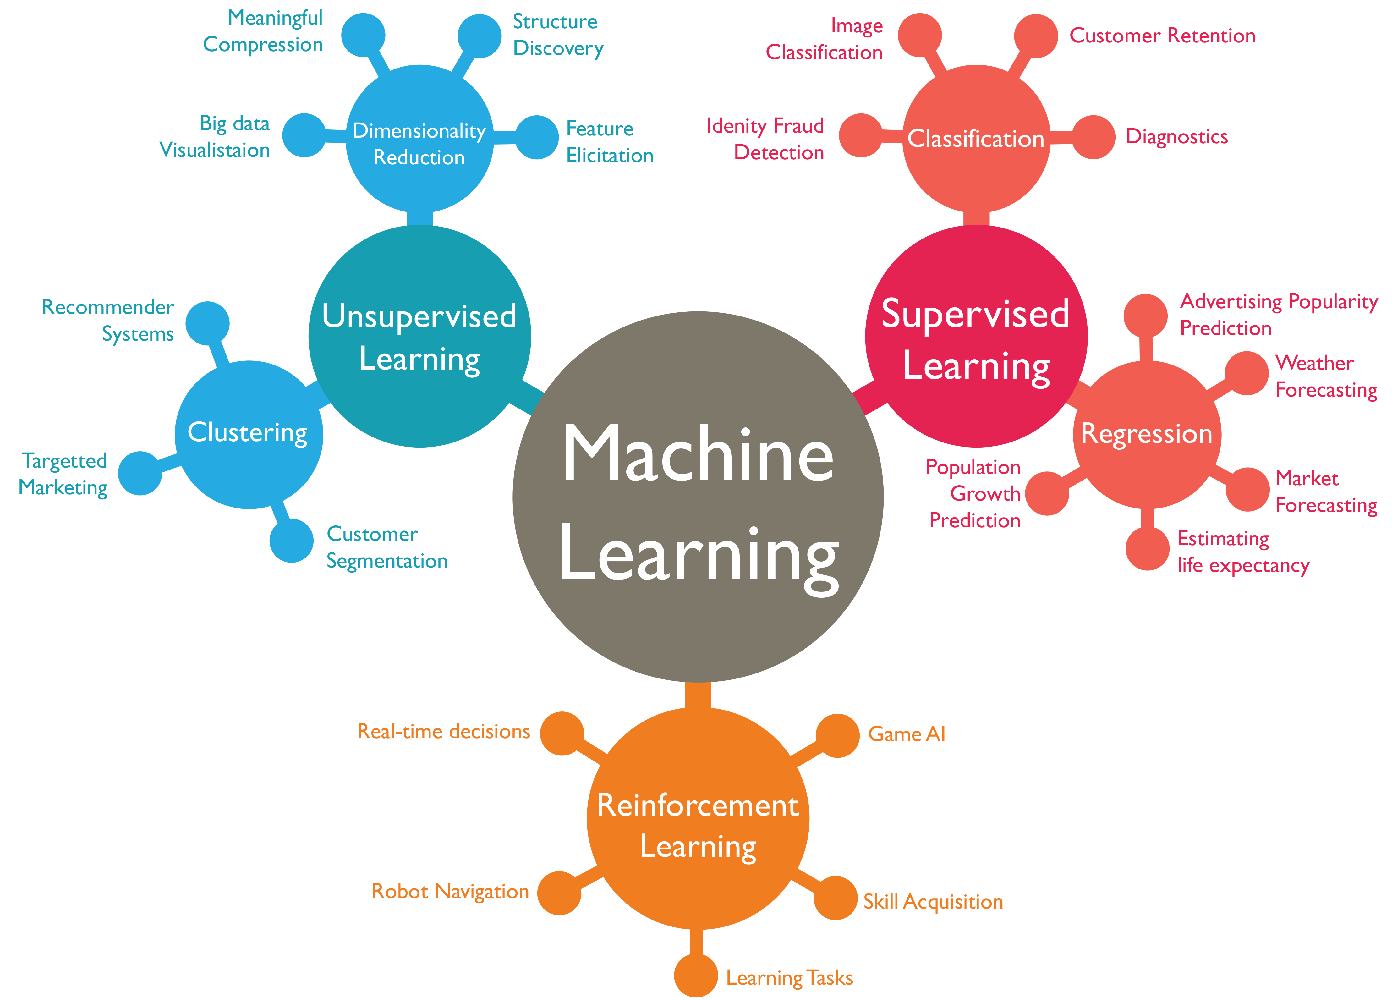
\includegraphics[width=\linewidth]{img/ml-soorten.png}
    \caption{Soorten machine learning met enklele toepassingen \autocite{Arroyo2017}}
    \label{fig:ml-soorten}
\end{figure}

\textcite{Lievens2019} schreef over 3 grote types binnen het domein van machine learning. Deze worden kort verklaard aan de hand van een praktisch voorbeeld. Figuur \ref{fig:ml-soorten} is een algemeen overzicht van wat hieronder beschreven is.


\subsubsection{Gesuperviseerd leren}
\label{subsubsec:gesuperviseerd-leren}

Bij gesuperviseerd leren probeert de software agent een functie te leren die een voorspelling maakt voor een gegeven input. De functie die deze voorspellingen maakt evolueert door het gebruik van een trainingsdataset met input-output waarden \autocite{Norvig1994}.

Classificatie is een typisch probleem dat opgelost wordt met gesuperviseerd leren, het wordt later in dit onderzoek op een andere manier opgelost. Het doel van classificatie is om aan de hand van enkele kenmerken een voorgedefinieerde klasse te voorspellen. Er wordt gesproken van een binair classificatieprobleem als er slechts 2 klassen zijn. Spamdetectie is hier een voorbeeld van. Door de belangrijke woorden uit een bericht te halen wordt er een attribuutvector opgebouwd. Door een model te trainen met duizenden berichten en als ze al dan niet spam zijn, kan het een voorspelling maken voor de gegeven vector \autocite{Lievens2019}.

\subsubsection{Ongesuperviseerd leren}
\label{subsubsec:ongesuperviseerd-leren}

Met ongesuperviseerd leren is het mogelijk om in een ongelabelde dataset patronen te vinden die eerder onbekend waren. Bij elke voospelling wordt voor elke categorie meegegeven hoe zeker het model is over zijn voorspelling \autocite{Hinton1999}.

Een ongelabelde dataset met gegevens over klanten waarvoor je te weten wilt komen als er onderliggende groepen ontdekt kunnen worden. Dit wordt ook clustering genoemd, een mogelijke oplossing is \autocite{Lievens2019}:

\begin{itemize}
    \item Klanten die waarschijnlijk hun contract verlengen.
    \item Ontevreden klanten die bijna zeker hun contract opzeggen.
    \item Klanten die voor een bepaalde aanbieding misschien hun contract verlengen.
\end{itemize}

Deze resultaten worden bekomen door berekeningen uit te voeren op de attribuutvector zonder een outputlabel. Deze techniek is, in het kader van dit onderzoek, minder relevant.

\subsubsection{Reinforcement Learning}
\label{subsubsec:reinforcement-learning}

Reinforcement learning focust zich op de acties die een software agent onderneemt om een zo hoog mogelijke beloning te krijgen. Er is dus geen nood aan een (gelabelde) dataset zoals bij gesuperviseerd en ongesuperviseerd leren. De agent probeert een balans te vinden tussen wat hij weet en wat er kan gebeuren \autocite{Kaelbling1996}. In essentie wil dit zeggen dat de agent probeert te leren welke acties leiden tot de hoogste totale beloning \autocite{Lievens2019}.

Deze techniek wordt verder besproken in het deel over geautomatiseerde machine learning.


Geautomatiseerde machine learning is het automatiseren van het trainingsproces bij een artificieel neuraal netwerk. De lage toegangsdrempel zorgt ervoor dat mensen met beperkte machine learning kennis sneller en simpeler een model kunnen trainen en gebruiken.

\subsubsection{Transfer Learning}
\label{subsubsec:transfer-learning}

\begin{figure}
    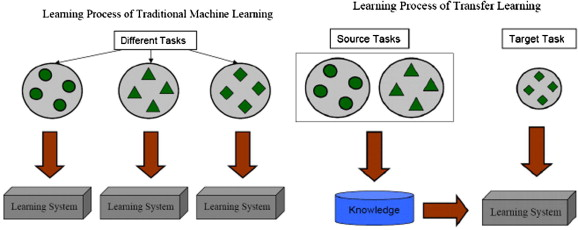
\includegraphics[width=\linewidth]{img/transfer-learning.jpg}
    \caption{Informatieoverdracht bij Transfer Learning \autocite{Pan2009}.}
    \label{fig:transfer-learning}
\end{figure}

Een andere manier om een neuraal netwerk te trainen is eerst een gegeneraliseerd model maken en die later specifiek toepassen op de situatie waarin het zich bevindt. Het idee achter transfer learning komt hierop neer, een gegeneraliseerd model kan vormen, kleurveranderingen en hoeken herkennen. Door de laatste lagen van het model af te knippen en nieuwe meer gespecialiseerde lagen toevoegt, zeg je in principe welke soort van de opgesomde eigenschappen het moet herkennen \autocite{Khandelwal2019}. 

In figuur \ref{fig:transfer-learning} is zichtbaar hoe een traditioneel model verschilt van een model getraind met transfer learning. Voor verschillende taken hoeft het niet volledig opnieuw getraind worden (op voorwaarde dat het binnen de generalisatie valt) en kan je de laatste lagen fine-tunen naar wens. Zo kan een model getraind worden om voertuigen te herkennen en later gespecialiseerd worden naar bijvoorbeeld auto's, vrachtwagens, fietsen of moto's.

\section{Neural Architecture Search}
\label{sec:nas}

\begin{figure}
    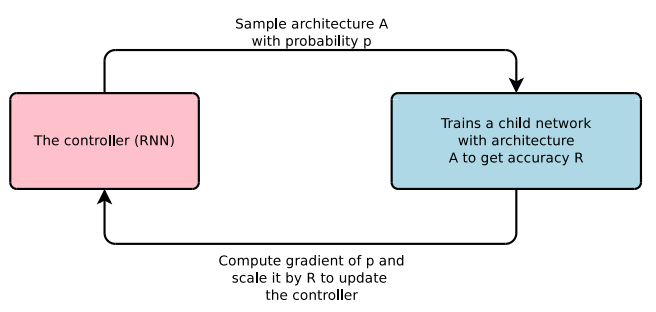
\includegraphics[width=\linewidth]{img/nas.png}
    \caption{Werking van Neural Architecture Search \autocite{ZophL2016}}
    \label{fig:nas-bp}
\end{figure}

Dergelijke geautomatiseerde machine learning systemen gebruiken een techniek die het ontwerp van een artificieel neuraal netwerk kan automatiseren, beter bekend als Neural Architecture Search \autocite{Elsken2019}. Uit \textcite{ZophL2016} wordt vastgesteld dat deze techniek een gelijkaardige of zelfs betere performantie heeft dan modellen die door een ML-ingenieur ontworpen zijn.

De technieken uit Sectie \ref{sec:hyperparameter-tuning} zijn onderliggend verwerkt en spelen een belangrijke rol binnen het domein van machine learning \autocite{ZophL2016}.

\subsubsection{Gebruik van Reinforcement Learning}

Neural Architecture Search gebruikt Reinforcement Learning om een model te trainen. Deze manier van werken is fundamenteel anders dan gesuperviseerd / ongesuperviseerd leren omdat het model niet beter wordt door het gebruik van datasets. Als alternatief kan het neuraal netwerk beloningssignalen herkennen waardoor het kan leren welke acties leiden tot een positief resultaat \autocite{Lievens2019}.

Op figuur \ref{fig:nas-bp} wordt gevisualiseerd hoe dit werkt. Op basis van controller structuur A (waarbij A een neuraal netwerk is) wordt een string met variabele lengte gegenereerd. Deze waarden worden gebruikt als hyperparameters om een kind-netwerk aan te maken, die getraind wordt met echte data en waarbij de accuraatheid gemeten wordt aan de hand van een validatie dataset. Het resultaat wordt gebruikt als beloningssignaal voor de controller, bij de volgende iteratie kunnen er hogere kansen gegeven worden aan parameters die leiden tot accurate voorspellingen \autocite{ZophL2016}. De controller zijn zoekfunctie zal dus verbeteren over tijd.

\section{Hyperparameter tuning}
\label{sec:hyperparameter-tuning}

In de vorige sectie is het gebruik van parameters aan bod gekomen. Neural Architecture Search en Hyperparameter tuning zijn dan ook sterk gerelateerd aan elkaar. De normale parameter bepalen het gedrag van een neuraal netwerk en hebben een grote invloed op het eindresultaat. Het gegeven gewicht aan een parameter stelt, zoals eerder vermeld, hoe groot de invloed is van deze laag / neuron op de voorspelling. \textcite{GoogleHT2020} verduidelijkt dat Hyperparameters eigen zijn aan de configuratie en niet aan het model. Zo moet er bepaald worden hoeveel lagen en het aantal neuronen per laag er zijn. Tijdens het trainen blijven deze constant. Volgens \textcite{Brust2019} zijn er verschillende manieren om de hyperparameters te optimaliseren. Brute force zal elke configuratie overlopen en beslissen hoe het model vordert terwijl feature selection gewichten aan verschillende hyperparameters geeft. Op die manier hebben vorige simulaties een impact bij de selectie van een nieuwe set parameters \autocite{Claesen2015}.

\textcite{ZophL2016} stelt dat deze methode in het algemeen minder goed werkt dan Neural Architecture Search, dit is omdat de netwerk configuraties gevormd worden in een zoekruimte met vaste lengte. Bayesian optimization \autocite{Bergstra2011}, een variant van hyperparameter tuning, werkt wel met variabele zoekruimtes maar blijven minder flexibel dan wat er voorgesteld wordt bij Neural Architecture Search \autocite{ZophL2016}.

\subsection{Bayesian optimization, meta-learning en ensemble construction}
\label{subsec:bayesian}

\subsection{Meta-learning}
\label{subsec:meta-learning}

\subsection{Ensemble construction}
\label{subsec:ensemble-construction}

\section{AutoML platformen}
\label{sec:automl-platformen}

\begin{figure}
    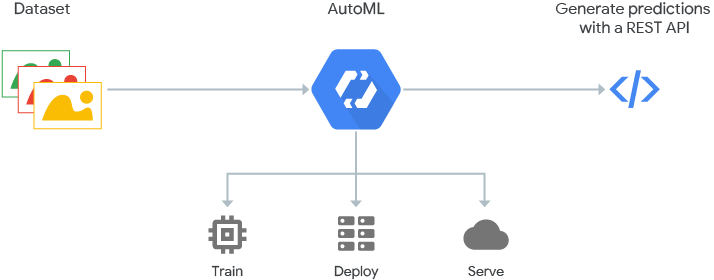
\includegraphics[width=\linewidth]{img/google-cloud-automl.png}
    \caption{Stappenplan voor een geautomatiseerd model in de cloud \autocite{Google2019}}
    \label{fig:google-cloud-automl}
\end{figure}

Het idee van geautomatiseerde toepassingen is niet nieuw, de evolutie van rekenkracht maakt het gewoon mogelijk. Er verschijnen allemaal nieuwe oplossing die runnen in de cloud of lokaal, al dan niet met grafische interfaces enzovoort. Op dit vlak is Google de koploper die het op een gebruiksvriendelijke manier aan de man brengt, maar programmeurs zijn vaak meer dan capabel om meer dan enkel een drag-en-drop systeem te gebruiken. Er zijn dan ook heel wat manieren die meer input vragen maar één bepaald aspect raken bij de gebruiker (open source, start-up, niet gecontroleerd door een groot bedrijf ...). . Met deze platformen probeert de industrie de kloof tussen machine learning en een doorsnee programmeur te dichten \autocite{Gutierrez2019}.

Een open source alternatief lijkt een goede oplossing, de interfaces zijn minder gebruiksvriendelijk dan een betalend product en er komt meer programmeerwerk aan te pas. Het resultaat is vaak commercieel bruikbaar zolang de restricties van de licentie gerespecteerd worden \autocite{Balter2015}. AutoKeras is een voorbeeld onder de MIT licentie, die geen commerciële restricties oplegt. Samen met AutoKeras zijn tpot en Auto Sklearn de best ondersteunde libraries.

In deze sectie worden enkele mogelijkheden besproken.

\subsection{Google Cloud AutoML}

Google Cloud AutoML zorgt voor een familiaire interface die een gebruiker snel op weg helpt. Naast Google hebben bedrijven zoals Microsoft en Amazon een platform gebouwd op hun respectievelijke cloud infrastructuur. De AutoML service kan voordelig zijn als het bedrijf al gebruik maakt van andere producten / diensten van de leverancier, extra kosten kunnen snel de lucht in gaan zonder toegang tot andere functies (bv. van Google Cloud) als dit niet het geval is. 

Zoals veel Google producten, heeft Cloud AutoML een familiaire interface die een gebruiker snel op weg helpt. Het proces is bijna even simpel als hun voorstelling in figuur \ref{fig:google-cloud-automl}, enkel het structureren van de dataset is niet opgenomen in de flow. De AutoML service heeft een goede kans om door te groeien in het bestaande platform van Google Cloud. De simultane werking tussen meerdere Cloud producten kan interessant zijn mocht het bedrijf gepartnered is met Google.

\subsection{AutoKeras}

Een AutoML systeem gebaseerd op Keras. De bedoeling van deze library is om machine learning toegankelijk te maken voor iedereen \autocite{jin2019}. AutoKeras is op dit moment nog in pre-release en kan nog sterk veranderen in de toekomst. Het gebruik is redelijk vanzelfsprekend en een volledige beschrijving van tekst en afbeeldingsanalyse zijn beschikbaar op de website. Van alle opgelijste mogelijkheden, vraagt deze library het meeste werk naast het voorzien van de data. Zo moet het model lokaal getraind worden en niet in de cloud, en moet de gebruiker een basis kennis Python hebben (om met de classifier van start te gaan). Een lokaal getraind model brengt ook wat voordelen met zich mee. Zo is er de mogelijkheid om het te exporteren naar een werkend Keras model dat nog verder aangepast kan worden. 

Voor de Image Classifier is het voorbeeld uitgewerkt met de MNIST Hand-Written Digits, zowat de standaard dataset voor afbeeldingsherkenning. Het bevat 70000 afbeeldingen van handgeschreven letters die voorzichtig opgeschoond zijn om te gebruiken als test. Ze worden vaak gebruikt bij het schrijven van de algoritmes om verbeteringen te verifiëren. Het gevolg hiervan is dat de behaalde nauwkeurigheid niet per se representatief is op realistische voorbeelden waar afbeeldingen verschillende resoluties, kleur-schalen en aspect-ratios kunnen hebben.

Het is aangewezen om het model te trainen op een machine met een externe grafische kaart die ondersteund wordt door de NVIDIA CUDA Toolkit.

\section{Deployment}

Voor een development team is het niet voldoende om enkel en alleen een model te trainen. Om het te kunnen gebruiken moet het ergens online staan zodat de applicatie waarin het verwerkt zit kan communiceren met het model. Bij de grote platformen zal het uitgerold worden op hun cloud services. Dat maakt nu eenmaal deel uit van hun kostenmodel. De gebruiker hangt dus in enigste zin vast aan zijn provider. 
In open source libraries is daar geen rekening mee gehouden. Een simpele oplossing is om zelf een REST API te schrijven. Er is geen beste manier omdat elke implementatie afhankelijk is van het export type van de library die je gebruikt. Om toch een representatief voorbeeld te geven wordt het deployment proces van een Keras model (export type van AutoKeras) besproken. 

Een goede strategie is om je API te bouwen in de taal waarin de library geschreven is. Zo kan je de bestaande interfaces van het geëxporteerde model direct aanspreken. In dit geval is het Python + Flask framework. Om het op een productie niveau te krijgen is het een goed idee om ook Redis te gebruiken\footnote{Redis is een gedistribueerde key-value store die volledige objecten in zijn geheugen kan opslaan en in deze situatie gebruikt wordt om wachtrijen te optimaliseren \autocite{Adrian2018}.}. Dan rest enkel nog de hosting, waardoor je soms toch uitkomt bij de grote platformen zoals Amazon AWS, Google Cloud Hosting enzovoort.

In \textcite{Adrian2018} is de volledige code te vinden om stap voor stap uit te voeren wat hierboven beschreven is.

%%=============================================================================
%% Methodologie
%%=============================================================================

\chapter{\IfLanguageName{dutch}{Methodologie}{Methodology}}
\label{ch:methodologie}

%% TODO: Hoe ben je te werk gegaan? Verdeel je onderzoek in grote fasen, en
%% licht in elke fase toe welke stappen je gevolgd hebt. Verantwoord waarom je
%% op deze manier te werk gegaan bent. Je moet kunnen aantonen dat je de best
%% mogelijke manier toegepast hebt om een antwoord te vinden op de
%% onderzoeksvraag.

Om tot een correct mogelijk resultaat te komen is het belangrijk om een grondige kennis te hebben van de geïmplementeerde algoritmen, modellen en platformen. Die zijn samen gebundeld tot een huidige stand van zaken en zijn terug te vinden in hoofdstuk \ref{ch:stand-van-zaken}.

Er werden meerdere prototypes opgezet die telkens volgens dezelfde criteria gequoteerd zijn. Verdere informatie over de gebruikte datasets is beschreven in sectie \ref{sec:datasets}. De vereisten waaraan elk systeem zo veel mogelijk aan moet voldoen worden toegelicht aan de hand van een requirements analyse in sectie \ref{sec:requirements}.

Het hoofddoel van dit onderzoek is ontdekken als de huidige staat van de technologie bruikbaar is in een bedrijfscontext zonder extreme operationele veranderingen. Dit kan afhangen van kosten om het systeem te gebruiken, extra mankracht die nodig is, eventuele omscholing enzovoort. De conclusie werd rond die vereisten geformuleerd. Omdat er verschillende implementaties getest zijn is het ook een vergelijkende studies en werden ze onderling tegen elkaar geëvalueerd. Dit niet alleen vanuit een technologisch standpunt (wat onderzocht werd in deze studie) maar ook de bijdrage die het levert aan de \textit{business value}. Om dit zo correct mogelijk te doen is in de achtergrond van de conclusie rekening gehouden met resultaten uit een studie vanuit een economisch standpunt. 

\section{Dataset}
\label{sec:datasets}

De keuze van de dataset is belangrijk. Dit onderzoek wil de capaciteiten van AutoML systemen testen op realistische situaties. De traditionele datasets (CIFAR, MNIST ...) waarmee deze algoritmen getraind zijn vallen onmiddellijk uit de selectie zoals uitgelegd in sectie \ref{subsec:autokeras}.

\subsection{Cats vs dogs}
\label{subsec:catsvsdogs}

\begin{figure}
    \begin{subfigure}{.5\textwidth}
        \centering
        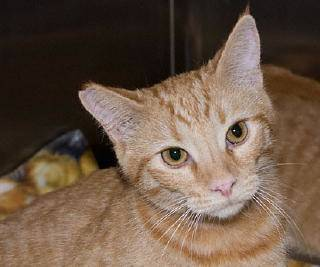
\includegraphics[width=.8\linewidth]{img/good_cat.jpg}
        \label{fig:cat-goog}
    \end{subfigure}%
    \begin{subfigure}{.5\textwidth}
        \centering
        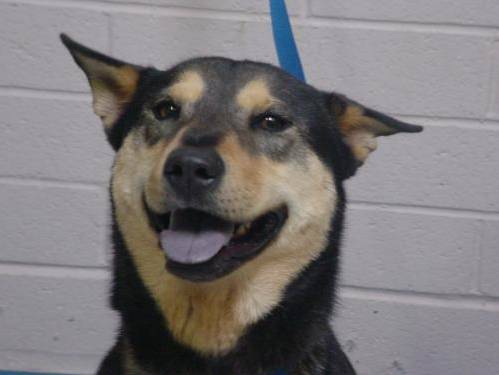
\includegraphics[width=.8\linewidth]{img/good_dog.jpg}
        \label{fig:dog-good}
    \end{subfigure}
    \caption{Kat en hond zijn de focus van de afbeelding.}
    \label{fig:catdog-good}
\end{figure}

\begin{figure}
    \begin{subfigure}{.5\textwidth}
        \centering
        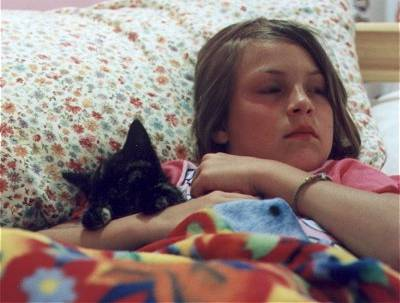
\includegraphics[width=.8\linewidth]{img/bad_cat.jpg}
        \label{fig:cat-bad}
    \end{subfigure}%
    \begin{subfigure}{.5\textwidth}
        \centering
        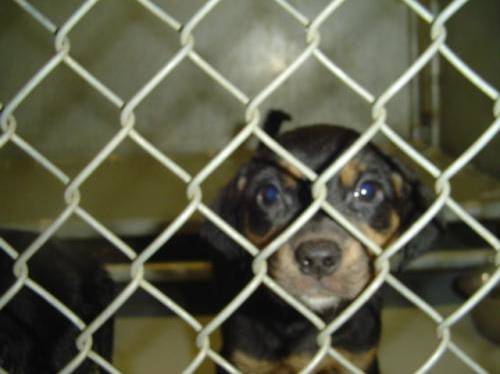
\includegraphics[width=.8\linewidth]{img/bad_dog.jpg}
        \label{fig:dog-bad}
    \end{subfigure}
    \caption{Kat en hond zijn niet de focus van de afbeelding.}
    \label{fig:catdog-bad}
\end{figure}

Alle systemen zijn getraind met een online\footnote{\url{https://www.kaggle.com/c/dogs-vs-cats/data}} dataset over katten en honden. Ooit was de dataset het onderwerp van een \textit{data science} wedstrijd en mogen vrij gebruikt worden. Het bestaat uit 250000 foto's die gelijkaardig zijn aan de afbeeldingen in figuur \ref{fig:catdog-good}. Er is niks van \textit{preprocessing} toegepast, de foto's kunnen dus evengoed op uw smartphone staan. Door realistische foto's te gebruiken introduceren we een nieuwe moeilijkheid voor de optimalisatiealgoritmen, zo moeten ze ook rekening houden met volgende zaken: 

\begin{itemize}
    \item Foto's kunnen zeer verschillende resoluties hebben
    \item De kleuren zijn in 3 dimensies (rood, groen, blauw)
    \item Door het originele formaat te behouden en de afbeelding niet te knippen naar het dier zelf, kan het zijn dat de focus van de afbeelding niet op het dier ligt (zie afbeeldingen in figuur \ref{fig:catdog-bad})
\end{itemize}

Onduidelijke foto's zijn in de minderheid maar handig om te ontdekken waaraan het model gevoelig is.

Omdat de \textit{dataset} gebruikt is in een wedstrijd zijn er honderden inzendingen beschikbaar van mensen die een poging gedaan hebben om het probleem op te lossen. Een vergelijking van performantie met onze geautomatiseerde modellen tegenover modellen die door een persoon zijn samengesteld is op zijn plaats.

\section{Requirementsanalyse}
\label{sec:requirements}

De verwachte functionaliteiten kunnen opgesplitst worden in twee categorieën. Enerzijds zijn er de functionele requirements die de gewenste functionaliteiten en het gedrag van een systeem beschrijven. Anderzijds de niet-functionele requirements, een oplijsting van kwaliteitseisen waaraan het moet voldoen.

\subsubsection{Functionele requirements}
\label{subsubsec:fr}

\begin{itemize}
    \item Ondersteuning voor verschillende resoluties van afbeeldingen
    \item Kan alle stappen uit het procesmodel uitvoeren (sectie \ref{sec:proces-model})
    \item Mogelijkheid om performantie te meten
    \item \textit{Batch} verwerking is ondersteund
\end{itemize}

\subsubsection{Niet-functionele requirements}
\label{subsubsec:nfr}

\begin{itemize}
    \item Moet snel kunnen \textit{deployen} naar een productieomgeving
    \item Performantie is vergelijkbaar met modellen die door een \textit{data scientist} gemaakt zijn
    \item Als ondersteunende technologie mag het niet duurder zijn dan een \textit{data scientist}
    \item Programmeurs met weinig of geen ervaring moeten het kunnen gebruiken
    \item Het resultaat kan ingebouwd worden in bestaande applicaties
\end{itemize}

Er is geen sprake van requirements die \textit{nice to have} of dergelijke zijn. Om te slagen moeten alle eisen in een bepaalde mate aanwezig zijn. Ze werden dan ook één voor één besproken. Op het einde van de hoofdstukken is een tabel voorzien die als overzicht van de requirements dient.


% Voeg hier je eigen hoofdstukken toe die de ``corpus'' van je bachelorproef
% vormen. De structuur en titels hangen af van je eigen onderzoek. Je kan bv.
% elke fase in je onderzoek in een apart hoofdstuk bespreken.

%%=============================================================================
%% AutoKeras
%%=============================================================================

\chapter{AutoKeras}
\label{ch:autokeras}

In dit hoofdstuk wordt het volledige AutoKeras proces uitgelegd. Dit door belangrijke stukken code te nemen en expliciet toe te lichten welke keuzes gemaakt zijn en waarom. Ook \textit{performance metrics} worden hier verzameld en vergeleken. Het model is met verschillende parameter configuraties getraind. Elke variant blijft wel hetzelfde code skelet gebruiken.

De ontwikkeling is volledig in \textit{Jupyter notebooks}\footnote{\url{https://jupyter.org/}} uitgewerkt. Om de code makkelijk lokaal te gebruiken is \textit{Anaconda Navigator\footnote{\url{https://docs.anaconda.com/anaconda/navigator/}}} aangeraden, de meeste \textit{packages} worden standaard mee geïnstalleerd. De code bevindt zich ook in Appendix \ref{ch:app:autokeras} en kan online bekeken worden\footnote{\url{https://github.com/robbedec/bachproef-automl}}.

Het is ook mogelijk om de notebook in de cloud uit te voeren. De dataset (omgezet naar een numpy array) en de notebooks kunnen direct geüpload worden naar Google Colab of Kaggle. De gebruiker heeft dan voor een bepaalde duur gratis toegang tot grafische kaarten.

Volgende \textit{packages} moeten zelf geïnstalleerd worden:

\begin{itemize}
    \item tensorflow-gpu (2.1.0)
    \item autokeras (1.0.2)
    \item graphviz (0.13.2)
\end{itemize}

\section{Voorafgaand werk}
\label{sec:autokeras-before}

\subsection{GPU activatie}
\label{subsec:autokeras-gpu}

Het verloop van de code is ook hoe je een model van nul kan trainen. Er wordt gewerkt met een \textit{CUDA integrated GPU}, om te testen als \textit{tensorflow} wel echt de GPU gebruikt kunnen er enkele commando's uitgevoerd worden. Als in de output een vermelding over de GPU staat mag u er vanuit gaan dat de die actief is. Meer informatie over CUDA drivers en hoe ze geïnstalleerd moeten worden is te vinden op de site van NVIDIA\footnote{\url{https://developer.nvidia.com/hpc}}.

\bigskip

\begin{python}
from tensorflow.python.client import device_lib

def get_available_devices():
    local_device_protos = device_lib.list_local_devices()
    return [x.name for x in local_device_protos]
print(get_available_devices()) 
\end{python}

Een mogelijkse output kan er als volgt uitzien: ['/device:CPU:0', '/device:GPU:0'].

Op de cloud platformen moeten geen speciale drivers geïnstalleerd worden maar enkel een \textit{accelerator} geactiveerd zijn in de \textit{notebook}.

\subsection{Data transformatie}
\label{subsec:autokeras-tranform}

De dataset bestaat deels uit een gelabelde afbeeldingen. Het bevat ook een verzameling ongelabelde afbeeldingen die tijdens de wedstrijd gebruikt werden als verificatie. In het kader van het onderzoek kunnen deze weggelaten worden en gaan we aan de slag met de gelabelde data. Elke afbeelding wordt genormaliseerd naar een standaard resolutie en omgezet naar een \textit{numpy array}\footnote{In de code is 'np' een verwijzing naar \textit{numpy}}. Dit zijn de kleurwaarden van elke pixel die samen een matrix vormen. Ook het label van de afbeelding is opgenomen in de matrix (0 = hond, 1 = kat). Momenteel staat alle data nog gegroepeerd volgens categorie. Voor de volgende stap is het belangrijk dat dit niet het geval is. Daarom wordt de matrix nog eens random gesorteerd.

Om consistentie tussen de experimenten te behouden wordt de matrix opgeslagen en bij een nieuwe configuratie terug ingeladen. De data transformatie wordt zo éénmaal uitgevoerd.

\bigskip

\begin{python}
def get_label(file):
    class_label = file.split('.')[0]
    if class_label == 'dog': label_vector = 0
    elif class_label == 'cat': label_vector = 1
    return label_vector
    
def get_data():
    data = []
    files = os.listdir(INPUT_PATH)
    
    for image in tqdm(files):
        label_vector = get_label(image)
        img = Image.open(INPUT_PATH + image).convert('L')
        img = img.resize((SIZE,SIZE))
    
        data.append([np.asarray(img),np.array(label_vector)])
        
    shuffle(data)
    return data

\end{python}

\section{Data preprocessing}
\label{sec:preprocessing-autokeras}

Een van de requirements is dat de \textit{preprocessing} voor de gebruiker gedaan wordt. Bij AutoKeras is dit niet 100\% het geval en moeten er zelf nog enkele zaken uitgevoerd worden. Zo moet de matrix die gemaakt is in sectie \ref{subsec:autokeras-tranform} opgedeeld worden in training en validatie datasets.

In \textit{data science} projecten wordt typisch x\_test en x\_train gebruikt om de \textit{features} van de afbeeldingen op te slaan, de matrix met pixel waarden. y\_test y\_train bevatten dan het bijhorend label. In de tweede stap wordt er dimensiereductie toegepast. De algoritmes houden geen rekening met kleuren dus die mogen we weglaten. De drie kleurendimensies (Rood, Groen, Blauw) worden omgezet naar één dimensie (grijswaarden). Deze conversie gebeurt in de laatste twee lijntjes van onderstaande code.

\bigskip

\begin{python}
x_train = np.array([data[0] for data in train], 'float32')
x_test = np.array([data[0] for data in test], 'float32')
y_train = [data[1] for data in train]
y_test = [data[1] for data in test]

x_train = np.array(x_train).reshape(-1,SIZE,SIZE,1)
x_test = np.array(x_test).reshape(-1,SIZE,SIZE,1)

x_train /= 255
x_test /= 255
\end{python}

\section{Model trainen en evalueren}
\label{sec:traineval-autokeras}

Na alle voorbereiding is het tijd om de \textit{classifier} in gang te steken. Hierbij moet enkel een naam (voor het uiteindelijke model) en het maximum aantal pogingen meegegeven worden. Op voorhand kan er niet ingesteld worden hoe lang er gezocht mag worden. Het is wel mogelijk dat het vroegtijdig beëindigd wordt (voor max. aantal pogingen bereikt is) omdat de \text{loss value} niet genoeg zakt over x-aantal iteraties.

Met de \pyth{clf.fit()} methode wordt het best passend model gekozen. Met de test dataset kan uiteindelijk de performantie van het model gemeten worden. \pyth{clf.evaluate()} geeft twee scores terug. Eerst de \textit{loss value}, het is een interpretatie die kijkt hoe goed het model scoort door training en test data te nemen. Let wel op dat de test dataset die wij definiëren enkel gebruikt wordt als \pyth{clf.evaluate()} uitgevoerd wordt. AutoKeras neemt van de trainings dataset standaard 20\% om te gebruiken als interne test data tijdens het trainen. De tweede waarde is het percentage van correct voorspelde afbeeldingen.

\bigskip

\begin{python}
clf = ak.ImageClassifier(max_trials=MAX_TRIES, name=OUTPUT_NAME)
clf.fit(x_train,y_train, verbose=2)

score = clf.evaluate(x_test, y_test)
\end{python}

Momenteel zit er een bug in het \textit{greedy} optimalisatie algoritme (dat standaard gebruikt wordt) van AutoKeras waardoor \textit{classifiers} met een max. aantal pogingen > 5 vroegtijdig beëindigd worden. Een voorlopige oplossing is om een de API van Automodel te gebruiken en zelf de instellingen te configureren. Achterliggend gebeurt dit ook als \pyth{ak.ImageClassifier()} geïnitialiseerd wordt. Als vervanging is er gekozen om \textit{random search} te gebruiken (zie sectie \ref{sec:hyperparameter-tuning}).

\bigskip

\begin{python}
clf = ak.AutoModel(
    inputs=[ak.ImageInput()], 
    outputs=[ak.ClassificationHead()], 
    tuner="random",
    max_trials=MAX_TRIES, 
    name=OUTPUT_NAME,
    overwrite=False
    )
    
clf.fit(x_train, y_train, verbose=2)
\end{python}

\section{Model visualisatie}
\label{sec:vis-autokeras}

\subsection{Confusion matrix}
\label{subsec:confusion-autokeras}

De \textit{confusion matrix} is waarschijnlijk één van de beste visualisaties om een inzicht in het model te krijgen. Voor elke categorie wordt het aantal juiste voorspellingen getoond maar ook het aantal afbeeldingen die aan de verkeerde categorie toegekend zijn. Een voorbeeld van een \textit{confusion matrix} is te vinden in afbeelding \ref{fig:confusion-matrices-autokeras}.

\bigskip

\begin{python}
plt.style.use('classic')
%matplotlib inline

mat = confusion_matrix(y_test, predictions.round())
labels = ['dog', 'cat']

sns.heatmap(mat.T, square=True, annot=True, fmt='d', cbar=False, xticklabels=labels, yticklabels=labels)
plt.xlabel('true category')
plt.ylabel('predicted category')
\end{python} 


\subsection{Verkeerde voorspellingen}
\label{subsec:wrong-predictions}

Om inzicht te krijgen in de verkeerde voorspellingen is het handig om die terug als afbeeldingen te tonen. Het kan een manier zijn om als persoon een patroon te vinden waartegen het model fouten maakt. Het zo gezegde ruis op de afbeeldingen. 

De eerste stap om voorspellingen op te splitsen is het interpreteren van de waarden. Zo krijg je bij een binair classificatieprobleem altijd een getal tussen 0 en 1 terug. Het kantelpunt is dan $\frac{1}{2}$, elke voorspelling die kleiner is wordt geclassificeerd als klasse 0 en alles groter als klasse 1. Om elke verkeerde voorspelling te zoeken kunnen we simpelweg het resultaat afronden en vergelijken met het bijhorend label.

\bigskip

\begin{python}
images = x_test.reshape(5000,64, 64)
incorrect_predictions = []

for i in range(0, len(predictions)):
    if predictions[i].round() != y_test[i]:
        incorrect_predictions.append(
            (i, images[i], predictions[i].round(4), y_test[i]))
\end{python}

In sectie \ref{sec:preprocessing-autokeras} zijn alle afbeeldingen omgezet naar grijswaarden. Als deze nu opnieuw geconverteerd worden zijn ze uiteraard zwart-wit foto's. Bij elke afbeelding wordt nog een legende gegenereerd. Zo is duidelijk te zien wat de index van de afbeelding is, wat de voorspelling van het model is (afgerond tot vier cijfers) en de werkelijke waarde.

\bigskip

\begin{python}
%matplotlib inline

figure, axes = plt.subplots(nrows=6, ncols=4, figsize=(16,16))

for axes, item in zip(axes.ravel(), incorrect_predictions):
    index, image, predicted, expected = item
    axes.imshow(image, cmap=plt.cm.gray_r)
    axes.set_xticks([])
    axes.set_yticks([])
    axes.set_title(f'index: {index}\np: {predicted}; e: {expected}')
    
plt.tight_layout()
\end{python}

Het resultaat van deze code is te zien in afbeelding \ref{fig:wrong-prediction-autokeras-5} en \ref{fig:wrong-prediction-autokeras-10}.

\subsection{Overzicht van de lagen}
\label{subsec:model-overview}

Het resultaat is een combinatie van Keras lagen (inputlagen, activatielagen, normalisatielagen...). Keras heeft een ingebouwde functie \pyth{model.summary()} die volgend resultaat oplevert:

\bigskip

\begin{python}
Model: "model"
_________________________________________________________________
Layer (type)                 Output Shape              Param #   
=================================================================
input_1 (InputLayer)         [(None, 64, 64, 1)]       0         
_________________________________________________________________
normalization (Normalization (None, 64, 64, 1)         3         
_________________________________________________________________
conv2d (Conv2D)              (None, 62, 62, 32)        320       
_________________________________________________________________
conv2d_1 (Conv2D)            (None, 60, 60, 64)        18496     
_________________________________________________________________
max_pooling2d (MaxPooling2D) (None, 30, 30, 64)        0         
_________________________________________________________________
dropout (Dropout)            (None, 30, 30, 64)        0         
_________________________________________________________________
flatten (Flatten)            (None, 57600)             0         
_________________________________________________________________
dropout_1 (Dropout)          (None, 57600)             0         
_________________________________________________________________
dense (Dense)                (None, 1)                 57601     
_________________________________________________________________
classification_head_1 (Sigmo (None, 1)                 0         
=================================================================
Total params: 76,420
Trainable params: 76,417
Non-trainable params: 3
_________________________________________________________________
\end{python}

Het overzicht kan ook geëxporteerd worden naar een afbeelding die beter geformatteerd is. De geëxporteerde afbeeldingen bevinden zich in Appendix \ref{ch:app:autokeras}.

\section{Resultaten}
\label{sec:results-autokeras}

Zoals eerder vermeld zijn er 2 modellen getraind met als enigste configuratieverschil, het maximum aantal pogingen. In andere woorden is dit het aantal verschillende Keras modellen dat aangemaakt mag worden. De resultaten van beide zijn samengevat in tabel \ref{table:autokeras-results}. 

Verder worden beide modellen vermeld als model A (max. 5 pogingen) en model B (max. 10 pogingen).

\begin{minipage}{\textwidth}
    De specificaties van het host systeem zijn:
    \begin{itemize}
        \item CPU: i7-7700HG
        \item GPU: Nvidia GeForce GTX 1050 Ti Max-Q
        \item RAM: 16GB
    \end{itemize}
\end{minipage}

\bigskip

\begin{table}[ht]
    \centering
    \begin{tabular}{c c c c c c} % centered columns (4 columns)
        \hline\hline %inserts double horizontal lines
        Max aantal pogingen & Accuracy & Loss & Trainingsduur & Aantal lagen \\ [0.5ex] % inserts table
        %heading
        \hline % inserts single horizontal line
        5   & 82.74\%   & 0.6383   & 2u    & 10 \\ 
        \hline %inserts single line
        10   & 81.37\%   & 0.7110   & 8u    & 10 \\ 
        \hline
    \end{tabular}
    \caption{Resultaten AutoKeras.}
    \label{table:autokeras-results}
\end{table}

\begin{figure}[b!]
    \centering
    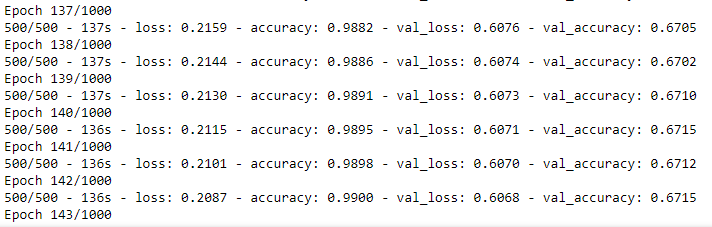
\includegraphics[width=\linewidth]{img/autokeras-overfit.png}
    \caption{Het model expres \textit{overfitten} in het kader van \textit{ensemble construction}.}
    \label{fig:autokeras-overfit}
\end{figure}

Wat meteen opvalt is dat een hoger aantal pogingen geen zekerheid is op betere prestaties. Zo wordt enkel de mogelijkheid gegeven op een uitgebreidere exploratie van de zoekruimte. Zo kan het algoritme bijvoorbeeld een extreem \textit{overfitted} model trainen in de hoop om die later te combineren met een andere om een beter resultaat te bekomen, een toepassing van \textit{ensemble construction} (zie sectie \ref{subsec:ensemble-construction}). Afbeelding \ref{fig:autokeras-overfit} komt rechtstreeks uit de output van model B en is niet te vinden in model A.

\begin{figure}[b!]
    \begin{subfigure}{0.5\textwidth}
        \centering
        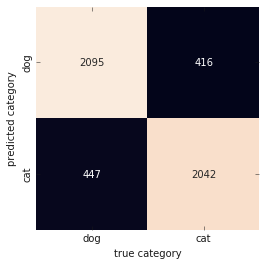
\includegraphics[width=0.8\linewidth]{img/autokeras-5-confusion.png}
        \caption{Max. pogingen = 5}
        \label{fig:confusion-autokeras-5}
    \end{subfigure}
    \begin{subfigure}{0.5\textwidth}
        \centering
        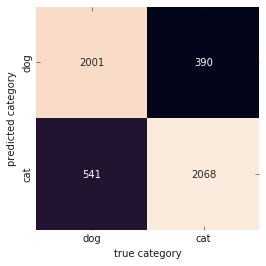
\includegraphics[width=0.8\linewidth]{img/autokeras-10-confusion.png}
        \caption{Max. pogingen = 10}
        \label{fig:confusion-autokeras-10}
    \end{subfigure}
    \caption{Overzicht confusion matrices}
    \label{fig:confusion-matrices-autokeras}
\end{figure}

\begin{minipage}{\textwidth}
De \textit{confusion matrices} in afbeelding \ref{fig:confusion-matrices-autokeras} tonen dat verspreiding van voorspellingen in beide gevallen redelijk overeen komt. Er is te zien dat model B meer aanleunt (en dus meer fouten maakt in die categorie) om kat te voorspellen dan hond, iets dat in model A in evenwicht is.
\end{minipage}

\begin{figure}
    \centering
    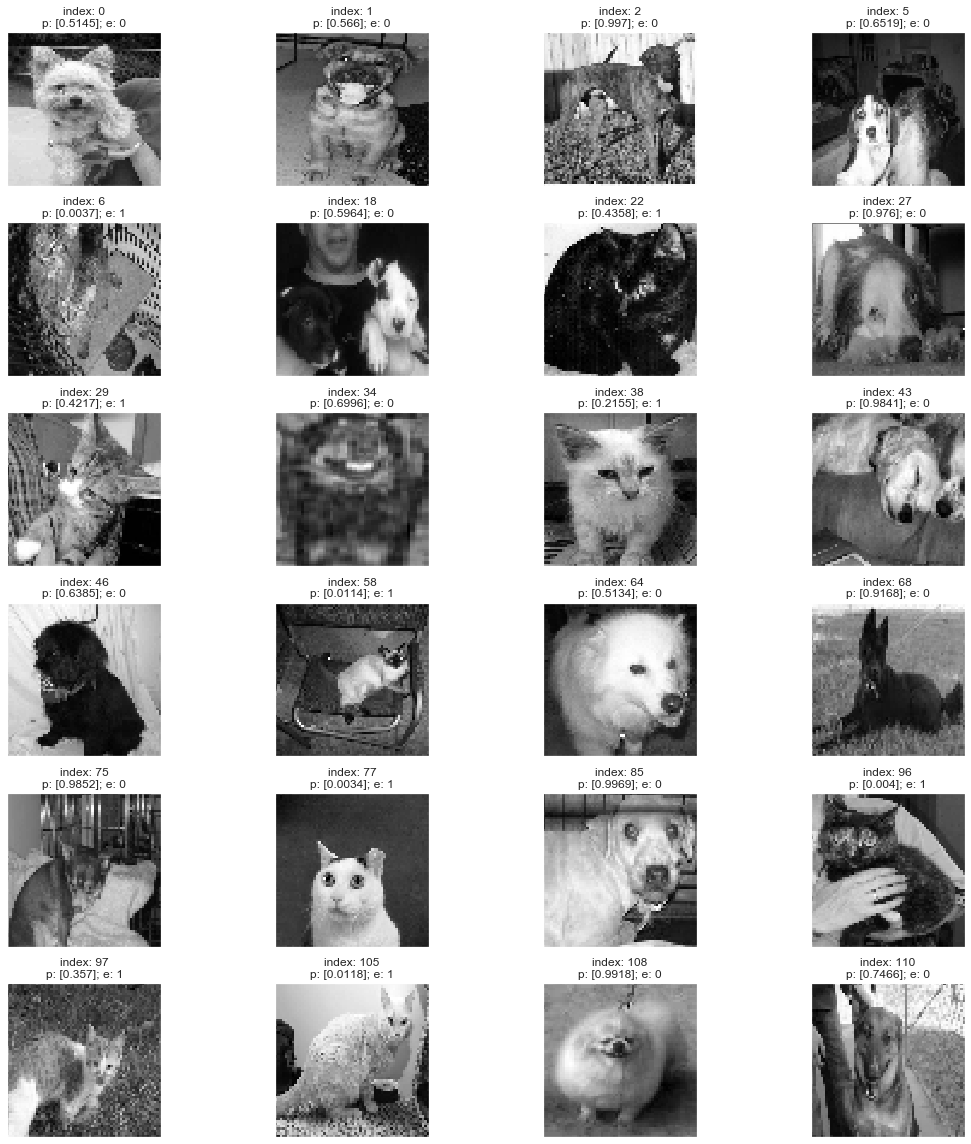
\includegraphics[width=\linewidth]{img/autokeras-5-wrong-images.png}
    \caption{Verkeerd voorspelde afbeeldingen van model A.}
    \label{fig:wrong-prediction-autokeras-5}
\end{figure}

\begin{figure}
    \centering
    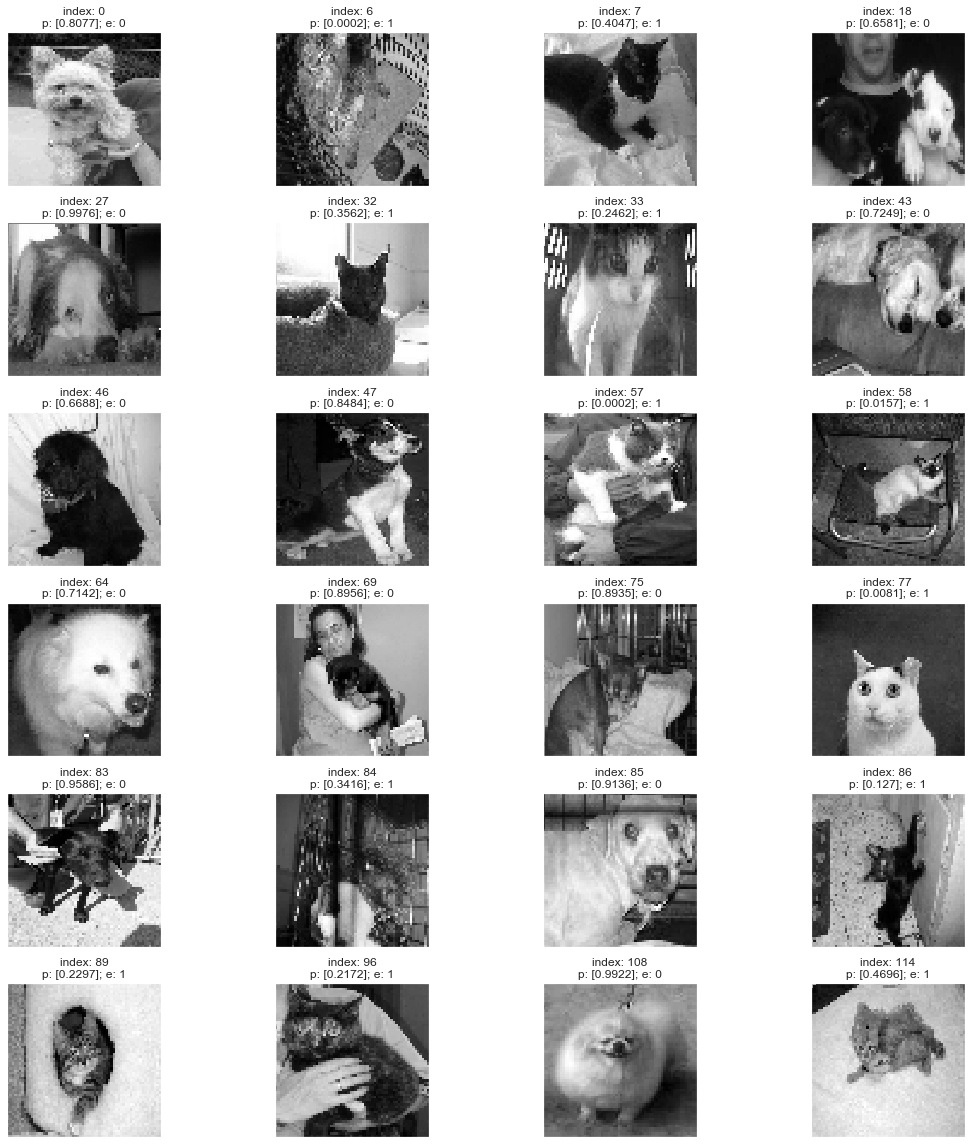
\includegraphics[width=\linewidth]{img/autokeras-10-wrong-images.png}
    \caption{Verkeerd voorspelde afbeeldingen van model B.}
    \label{fig:wrong-prediction-autokeras-10}
\end{figure}

Van beide modellen zijn 24 verkeerd voorspelde afbeeldingen gevisualiseerd (zie Figuren \ref{fig:wrong-prediction-autokeras-5} en \ref{fig:wrong-prediction-autokeras-10}). Bij sommige afbeelding kan duidelijk afgeleid worden wat de oorzaak is, mensen of andere onbekende objecten op de foto's. Andere zijn moeilijker te verklaren. Voor nu kan er besloten worden dat het model waarschijnlijk moeite heeft met de gespitste oren. Een typisch kenmerk van katten maar het komt soms ook voor bij honden. Maar ook het feit dat soms het volledige lichaam afgebeeld is en soms maar een deel van het hoofd.

Met een gemiddelde score van 82\% bekomen we een goed resultaat als er rekening gehouden wordt met de beperkte hoeveelheid \textit{data preprocessing}. Om dit op productie niveau te krijgen moet er wel meer moeite gedaan worden om de trainingsdataset beter te verwerken. Handgemaakte modellen uit de competitie behalen scores tot 98\%\footnote{\url{https://www.kaggle.com/c/dogs-vs-cats/leaderboard}}.

Tijdens het trainingsproces heeft de aanwezigheid van een TPU geen invloed op de snelheid. Deze wordt gewoonweg niet gebruikt. Een TPU of \textit{tensor processing unit} is een schakeling van \textit{accelerators} die het proces vele malen sneller uitvoert. AutoKeras bied op dit moment geen ondersteuning om deze te gebruiken waardoor er teruggevallen wordt op de GPU's. De afwezigheid vormt wel een nadeel aangezien TPU's verder uitgroeien tot de nieuwe industrie standaard.

Voor een open-source library zit er zeker potentieel in voor de toekomst als u weet dat op een gelijkaardig niveau van \textit{preprocessing} en dezelfde dataset, een pre-release versie van AutoKeras slechts 67\% behaalde \autocite{Chopra2019}.

\section{Requirements}

\subsection{Functionele requirements}
\label{subsec:autokeras-fr}

\subsubsection{Implementatie van het procesmodel}
\label{sucsubsec:autokeras-fr-procesmodel}

Er is geen sprake van een volledige implementatie. Als open source project dient het in de eerste plaats als een onderzoeksproject. AutoKeras is simpelweg hun contributie aan de \textit{state of the art}. Niet commercieel onderzoek heeft weinig last van economische druk waardoor nieuwe \textit{features} soms lang op zich laten wachten. 

Bij AutoKeras moet \textit{data preprocessing} zelf uitgevoerd worden. De optimalisatiealgoritmen gaan zelf de belangrijke \textit{features} zoeken en selecteren. Dit houdt in dat de data getransformeerd moet worden (numpy array in de juiste dimensies), opgesplitst en aangepast volgens de intenties van de gebruiker vooraleer het gebruikt kan worden door \pyth{ImageClassifier()}.

\subsubsection{Beschikbare metrics}
\label{sucsubsec:autokeras-fr-metrics}

De output van het algoritme wordt geëxporteerd naar een gecompileerd Keras model, onderling gebruikt het ook Keras lagen. Dit wil zeggen dat alle mogelijke visualisaties van Keras perfect mogelijk zijn met de output. In het experiment gaat het dan vooral over \pyth{model.summary()} en gelijkaardige output die ons een inkijk in het resultaat geeft.

Omdat de ruwe resultaten ook beschikbaar zijn, is de gebruiker vrij om andere \textit{packages} te gebruiken. Zo kan met een lijst voorspellingen een \textit{confusion matrix} gemaakt worden aan de hand van de scikit-learn \textit{library}. De array van grijswaarden kan ook terug omgezet worden naar afbeeldingen om bijvoorbeeld, verkeerde voorspellingen te tonen. Alle verschillende mogelijkheden zijn enkel begrensd door het aantal beschikbare \textit{packages}.

Met de wiskundige formules kunnen ook allemaal verschillende statistieken berekend worden.

\subsubsection{Batch verwerking}
\label{sucsubsec:autokeras-fr-batch}

Voor een AutoKeras \textit{classifier} bestaat op de \pyth{ImageClassifier.fit()} methode een \textit{batch\_size} argument die dit kan manipuleren. Deze optie bepaalt hoeveel afbeeldingen er bij elke iteratie gepropageerd worden door het model. Door \textit{mini batches} te gebruiken moeten niet alle afbeeldingen op hetzelfde moment in het geheugen van de computer geladen worden. Onderliggend gebeuren er meer updates aan de \textit{gradient} die tot betere resultaten kunnen leiden.

\subsection{Niet-functionele requirements}
\label{subsec:autokeras-nfr} 

\subsubsection{Deployment}
\label{sucsubsec:autokeras-nfr-deployment}

Om een model online te krijgen is ook hier niet voorzien. Als gebruiker ben je zelf verantwoordelijk om de benodigde infrastructuur te voorzien. Ook zijn er mogelijks uitbreidingen nodig om de implementatie op productieniveau te krijgen. Meer informatie hierover in sectie \ref{sec:deployment}.

\subsubsection{Performantie}
\label{sucsubsec:autokeras-nfr-performantie}

Het uiteindelijke resultaat in ons experiment is bruikbaar. Met 83\% is de technologie op zich bewezen. Betere resultaten hangen sterk af van de hoeveelheid en kwaliteit van de \textit{data preprocessing}.

\subsubsection{Kostprijs}
\label{sucsubsec:autokeras-nfr-price}

Het gebruik van de \textit{library} zelf is volledig gratis. Ook voor het resultaat moet niet betaalt worden. Er moet zelf gekozen worden over welke investeringen gedaan worden in verband met de infrastructuur (aantal GPU's, kloksnelheid, elektriciteit ... ). Op zich kan een model getraind worden op een (gratis) online platform zoals Kaggle, of Google Colab. Om langere GPU tijden te verkrijgen kan een pro account aangeschaft worden.

\subsubsection{Verwerking}
\label{sucsubsec:autokeras-nfr-verwerking}

Omdat de meeste \textit{wrappers} geschreven zijn in Python, is het een goede keuze om er een eigen API mee te maken. Voor Flask zijn er online zeer veel \textit{tutorials} beschikbaar. Ook hierover is meer informatie te vinden in sectie \ref{sec:deployment}.
%%=============================================================================
%% Google AutoML
%%=============================================================================

\chapter{Google Cloud AutoML}
\label{ch:google-automl}

Google Cloud AutoML is zoals de naam zegt, deel van het Cloud platform. In dit hoofdstuk wordt gebruik gemaakt van een \textit{storage server} en de \textit{vision API}. Om toegang te krijgen is uiteraard een account nodig, en als nieuwe gebruiker is er \$300 beschikbaar die vrij gespendeerd kan worden op het platform (binnen de periode van één jaar).

De interfaces zijn zeer gebruiksvriendelijk en maken vaak gebruik van drag en drop systemen. 

Vooraleer er gestart kan worden is een korte setup op zijn plaats. De volledige code van het gebruikte \textit{jupyter notebook} is te vinden in Appendix \ref{ch:app:google-automl}.

\section{Voorafgaand werk}
\label{sec:google-automl-before}

\subsection{Google Cloud Data Storage}
\label{subsec:google-cloud-data-storage}

Om de \textit{computer vision API} te gebruiken moeten de afbeeldingen geüpload worden. Dit kan rechtstreeks in batches van max. 30 MB. Met de hoeveelheid afbeeldingen die gebruikt worden in dit onderzoek is dit niet praktisch. Voor grote hoeveelheden data kan daarom een online bucket gebruikt worden. De afbeeldingen bevinden zich dan op een \textit{data storage server} van Google Cloud.

De indeling van de data moet er als volgt uitzien:

\dirtree{%
    .1 online bucket.
    .2 cat.
    .3 cat.0.jpg.
    .3 cat.1.jpg.
    .3 cat.2.jpg.
    .2 dog.
    .3 dog.0.jpg.
    .3 dog.1.jpg.
    .3 dog.2.jpg.
}

Dit is belangrijk voor de volgende stap. Op deze manier kunnen er makkelijk labels toegekend worden aan de afbeeldingen. Dit op een manier die het platform kan interpreteren.

\subsection{Structuur van de data}
\label{subsec:google-structure}

Nu alle data online beschikbaar is, moet er nog een overzicht gecreëerd worden. Aan de hand van een \textit{jupyter notebook} wordt een csv gemaakt die voor elke afbeelding, de locatie op Google Cloud Storage en het bijhorend label bevat. Alle niet afbeeldingen worden uit de map gefiltered

\begin{python}
data_array = []

for (dict_key, files_list) in files_dict.items():
    for filename in files_list:
        if '.jpg' not in filename:
            continue # don't include non-photos
            
        label = dict_key
        data_array.append((base_gcs_path + dict_key + '/' + filename , label))

\end{python}

Nu moet \pyth{data_array} enkel nog ingeladen worden in een \textit{pandas dataframe}. In de \textit{pandas library} zit een functie die een dataframe kan opslaan als een csv bestand. Merk op dat de indexes van de kolommen en rijen niet mee opgeslagen worden. Deze kunnen als \pyth{False} geflagged worden in de functie.

\pyth{dataframe.to_csv('all_data.csv', index=False, header=False)}

De output van het csv bestand zou er als onderstaand uit moeten zien. Natuurlijk met een andere bucket naam.

gs://rdc-automl-catsvsdogs/dog/dog.100.jpg dog \\
gs://rdc-automl-catsvsdogs/dog/dog.1000.jpg dog \\
… … … \\
gs://rdc-automl-catsvsdogs/cat/cat.9995.jpg cat \\
gs://rdc-automl-catsvsdogs/cat/cat.9996.jpg cat
\\

Het csv bestand moet dan ook toegevoegd worden aan de bucket.

\section{Model trainen en evalueren}
\label{sec:google-automl-train}

Om het trainen te starten moet nu enkel het csv bestand (dat op Google Cloud Storage) staat selecteren. Vervolgens worden alle afbeeldingen geïmporteerd en opgesplitst in training, validatie en testen. In ons geval van 25000 afbeeldingen worden ze als volgt opgesplitst.

\begin{itemize}
    \item Training: 10000
    \item Validatie: 5000
    \item Testen: 5000
\end{itemize}

Elke dataset is gelijk verdeeld over de twee categorieën. Als er dus over 10000 afbeeldingen gesproken worden, zijn het in feite 5000 katten en 5000 honden.

\section{Model visualisatie}
\label{sec:google-automl-visualisation}

\section{Deployment}
\label{sec:google-automl-deployment}

Zoals besproken in sectie \ref{subsubsec:client-library} kunnen er interacties zijn via een \textit{client library}. De code kan oftewel intern in de applicatie verwerkt worden (indien de code geschreven is in Python). Een tweede manier is om de het Python script extern op te slaan en op te roepen als het nodig is.

\bigskip

\begin{python}
import sys

from google.cloud import automl_v1beta1
from google.cloud.automl_v1beta1.proto import service_pb2


# 'content' is base-64-encoded image data.
def get_prediction(content, project_id, model_id):
    prediction_client = automl_v1beta1.PredictionServiceClient()
    
    name = 'projects/{}/locations/us-central1/models/{}'.format(project_id, model_id)
    payload = {'image': {'image_bytes': content }}
    params = {}
    request = prediction_client.predict(name, payload, params)
    return request  # waits till request is returned

if __name__ == '__main__':
    file_path = sys.argv[1]
    project_id = sys.argv[2]
    model_id = sys.argv[3]

    with open(file_path, 'rb') as ff:
        content = ff.read()
    
    print get_prediction(content, project_id, model_id)
\end{python}

De functie verwacht drie argumenten. Een afbeelding (geëncodeerd in base-64), het project\_id en het model\_id. De ID's zijn te vinden in de eigenschappen van het project en model op Google Cloud.

\bigskip

\begin{python}
python predict.py YOUR_LOCAL_IMAGE_FILE 156243918112 ICN8843552342109323264
\end{python}

\begin{figure}
    \centering
    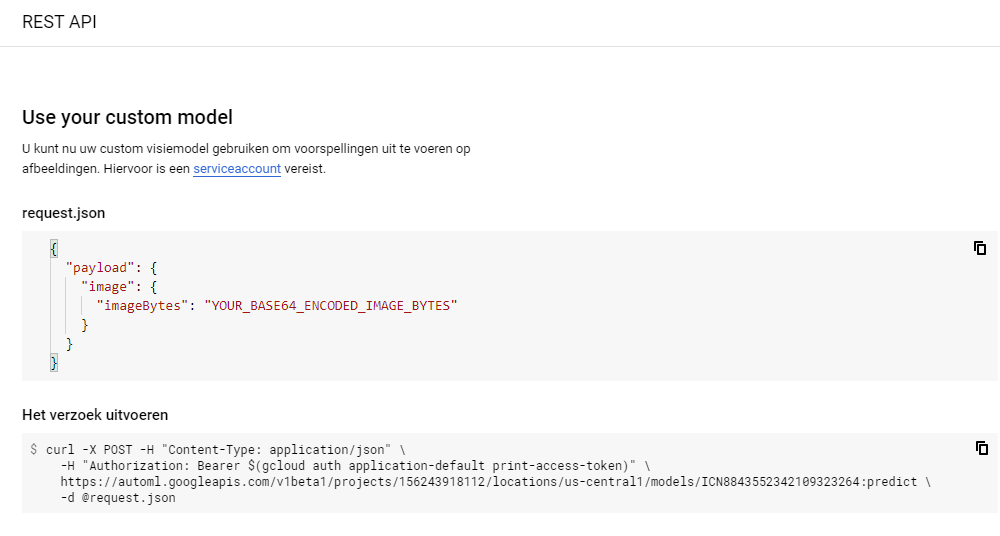
\includegraphics[width=\linewidth]{img/google-automl-rest.png}
    \caption{Requests sturen naar de REST API van Google AutoML.}
    \label{fig:google-automl-rest}
\end{figure}

Als een model gedeployed is, wordt er standaard een REST service aangemaakt. De gebruiker kiest dan zelf om een wrapper te schrijven (om een familiaire interface te maken) of om de requests met curl door te sturen, zoals op afbeelding \ref{fig:google-automl-rest}. 


\section{Requirements}
\label{sec:google-requirements}

%\input{...}
%\input{...}
%...

%%=============================================================================
%% Conclusie
%%=============================================================================

\chapter{Conclusie}
\label{ch:conclusie}

% TODO: Trek een duidelijke conclusie, in de vorm van een antwoord op de
% onderzoeksvra(a)g(en). Wat was jouw bijdrage aan het onderzoeksdomein en
% hoe biedt dit meerwaarde aan het vakgebied/doelgroep? 
% Reflecteer kritisch over het resultaat. In Engelse teksten wordt deze sectie
% ``Discussion'' genoemd. Had je deze uitkomst verwacht? Zijn er zaken die nog
% niet duidelijk zijn?
% Heeft het onderzoek geleid tot nieuwe vragen die uitnodigen tot verder 
%onderzoek?

In eerste instantie werd er (indirect) onderzocht als zo'n ingewikkeld proces wel geautomatiseerd kan worden. De resultaten tonen aan dat AutoML wel degelijk een plaats verdient in de wereld van \textit{machine learning}. De hoofdvraag blijft natuurlijk de bruikbaarheid voor bedrijven en daar zijn toch enkele opmerkingen over. Zo zal er zeker een afweging plaatsvinden waarbij kwaliteit tegenover kost wordt gezet. AutoML is niet goedkoop, zeker op een cloud platform dat snel drie à vierduizend euro per maand kan kosten om operationeel te blijven. Voor AutoKeras zijn de kosten op het eerste zicht beperkt tot verbruikte elektriciteit en \textit{deployment}. Men moet daarbij rekening houden dat elke stap zelf geprogrammeerd moet worden en er toch enige kennis voor nodig is. Het uiteindelijk resultaat wordt dan deels bepaald door de \textit{data preprocessing} die ook handmatig moet gebeuren, deze stap is een belangrijke \textit{trigger} om hoge scores te behalen zoals bij Google Cloud AutoML.

Beide systemen komen de verwachtingen na maar moeten op de juiste plaats ingezet worden. Zo is Google Cloud AutoML een volwaardig \textit{drop in replacement} in bestaande applicaties. Het proces kan niet eenvoudiger zijn en de verschillende manieren om het te integreren zorgen ervoor dat het in meeste situaties past. AutoKeras, in zijn huidige staat, is niet verfijnd genoeg om productie waardig te zijn. De extra moeite om de eerste stappen van het procesmodel te verbeteren kan evengoed verwisseld worden met een ML-ingenieur die het volledige proces uitvoert. Die niche kennis blijft noodzakelijk om te slagen. Anderzijds blijkt het wel een goede \textit{tool} te zijn in de gereedschapskist van ML-ingenieurs enzovoort. Stel een situatie voor waarbij zo snel mogelijk een MVP\footnote{Minimum viable product} voorgesteld moet worden. Zonder al te veel moeite kan er met AutoKeras een basis gelegd worden, ook kan het een andere inkijk over het probleem geven die misschien nog niet overwogen was. 

Let wel op, Google Cloud AutoML heeft ook zijn nadelen. Naast het stevig kostenplaatje is er ook nog de \textit{vendor lock in} op de cloud. Zo werd er voor een kleine toepassing al gebruik gemaakt van \textit{storage servers}, \textit{vision API} en een \textit{deployment platform}. Als klant is het niet de bedoeling dat een applicatie volledig afhankelijk is van één platform. Het neemt deels de vrijheid af, zo is het niet mogelijk om de structuur van het model te zien. 

De toekomst van geautomatiseerde \textit{machine learning} ziet er alvast goed uit. De verbeteringen tussen versies van AutoKeras vallen op en ook steeds meer cloud platformen bieden een gelijkaardige service aan. Er is een echte \textit{push} aan de gang, van de \textit{community} en de bedrijven, om de toepassingen toegankelijker te maken. Verder onderzoek over dit onderwerp zou zich kunnen richten op individuele stappen van het procesmodel, bijvoorbeeld de \textit{data preprocessing}. De automatisatie ervan is niet vanzelfsprekend omdat dit voor elke dataset anders is.

%%=============================================================================
%% Bijlagen
%%=============================================================================

\appendix
\renewcommand{\chaptername}{Appendix}

%%---------- Onderzoeksvoorstel -----------------------------------------------

\chapter{Onderzoeksvoorstel}

Het onderwerp van deze bachelorproef is gebaseerd op een onderzoeksvoorstel dat vooraf werd beoordeeld door de promotor. Dat voorstel is opgenomen in deze bijlage.

% Verwijzing naar het bestand met de inhoud van het onderzoeksvoorstel
%---------- Inleiding ---------------------------------------------------------

\section{Introductie} % The \section*{} command stops section numbering
\label{sec:introductie}

Machine learning en eenvoudig in dezelfde zin gebruiken, geen vanzelfsprekende opdracht maar wel iets dat Google probeert te realiseren. Met eigenschappen op hun site \autocite{Google2019} zoals: Uitstekende prestaties; Snel aan de slag; ontstaan er met Cloud AutoML toch enkele mogelijkheden om als programmeur (zonder professionele AI kennis) machine learning diensten te voorzien in een applicatie zonder dat er een data scientist bij het project betrokken wordt. Dit onderzoek, gefocust op het classificeren en herkennen van afbeeldingen, probeert aan te tonen dat deze service bruikbaar is voor bedrijven en hoe het scoort tegenover alternatieven.

%---------- Stand van zaken ---------------------------------------------------

\section{Literatuurstudie}
\label{sec:literatuurstudie}

% Voor literatuurverwijzingen zijn er twee belangrijke commando's:
% \autocite{KEY} => (Auteur, jaartal) Gebruik dit als de naam van de auteur
%   geen onderdeel is van de zin.
% \textcite{KEY} => Auteur (jaartal)  Gebruik dit als de auteursnaam wel een
%   functie heeft in de zin (bv. ``Uit onderzoek door Doll & Hill (1954) bleek
%   ...'')

Geautomatiseerde machine learning is het automatiseren van het trainingsproces bij een artificieel neuraal netwerk. De lage toegangsdrempel zorgt ervoor dat mensen met beperkte machine learning kennis sneller en simpeler een model kunnen trainen en gebruiken.

\subsection{Achterliggende werking}

\begin{figure}
    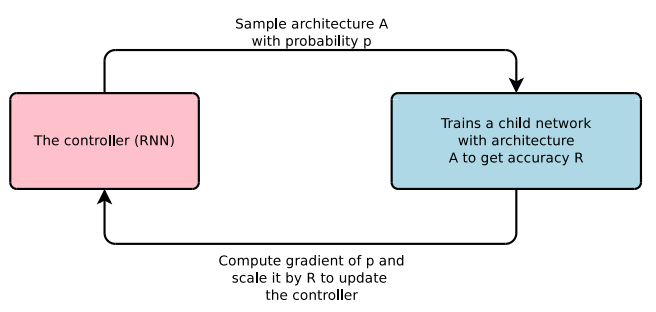
\includegraphics[width=\linewidth]{img/nas.png}
    \caption{Werking van Neural Architecture Search}
    \label{fig:nas}
\end{figure}

Dergelijke AutoML systemen gebruiken een techniek die het ontwerp van een artificieel neuraal netwerk kan automatiseren, beter bekend als Natural Architecture Search \autocite{Elsken2019}. Uit \textcite{ZophL2016} wordt vastgesteld dat deze techniek een gelijkaardige of zelfs betere performantie heeft dan modellen die door een ML-ingenieur ontworpen zijn.

Natural Architecture Search gebruikt Reinforcement Learning om een model te trainen. Deze manier van werken is fundamenteel anders dan gesuperviseerd / ongesuperviseerd leren omdat het model niet beter wordt door het gebruik van datasets. Als alternatief kan het neuraal netwerk beloningssignalen herkennen waardoor het kan leren welke acties leiden tot een positief resultaat \autocite{Lievens2019}.

Op figuur \ref{fig:nas} wordt gevisualiseerd hoe dit werkt. Op basis van controller structuur A (waarbij A een neuraal netwerk is) wordt een string met variabele lengte gegenereerd. Deze waarden worden gebruikt als parameters om een kind-netwerk aan te maken, die getraind wordt met echte data en waarbij de accuraatheid gemeten wordt aan de hand van een validatie dataset. Het resultaat wordt gebruikt als beloningssignaal voor de controller, bij de volgende iteratie kunnen er hogere kansen gegeven worden aan parameters die leiden tot accurate voorspellingen \autocite{ZophL2016}. De controller zijn zoekfunctie zal dus verbeteren over tijd.



\subsection{Gelijkaardige tools}
sdfq

%---------- Methodologie ------------------------------------------------------
\section{Methodologie}
\label{sec:methodologie}

Eerst en vooral wordt er een image dataset gemaakt die gebruikt wordt om de modellen te trainen en te valideren. Om een model te trainen is er een grote hoeveelheid data nodig. FFmpeg is een tool waarmee je de frames van een video (in dit geval een 360 graden video van het object) kan opsplitsen in afbeeldingen. De classificatie van de images wordt verwerkt met pandas, een data-analyse library voor Python.

Voor het experiment worden 2 modellen getraind met Google Cloud AutoML en AutoKeras. Zo kan het resultaat vergeleken worden met een open source alternatief. 

Er worden een aantal afbeeldingen geselecteerd van verschillende moeilijkheidsgraden om de modellen te toetsen.

%---------- Verwachte resultaten ----------------------------------------------
\section{Verwachte resultaten}
\label{sec:verwachte_resultaten}

\begin{figure}
    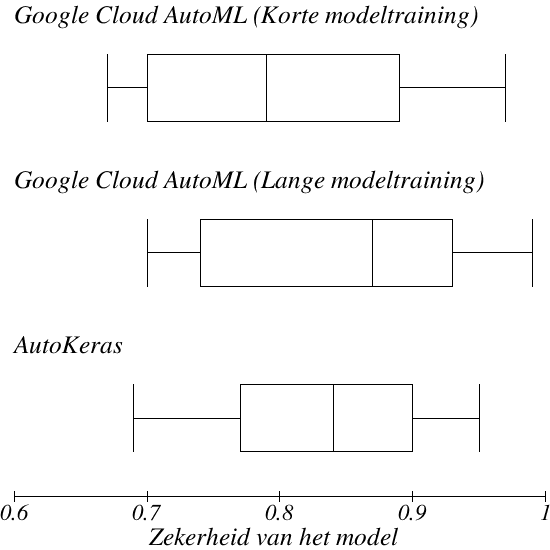
\includegraphics[width=\linewidth]{img/boxplot.png}
    \vspace{1mm}
    \caption{Verwachte correctheid van de modellen}
    \label{fig:boxplot1}
\end{figure}

Er worden goede resultaten verwacht van Google Cloud AutoML. Je betaalt voor een service en dan wil de gebruiker positieve resultaten op tafel zien. De trainingsduur van het Google Cloud AutoML model zal ook een zichtbare en positieve impact hebben op de gemiddelde score van een afbeelding. Uit het verleden hebben we geleerd dat \emph{community driven development} vaak leidt tot een performant resultaat (bv. de niet automatische versie, Keras) dat door veel developers onderhouden wordt. Voor een bedrijf is dit zeer interessant vanwege het kostenplaatje dat volledig wegvalt voor het gebruik van de technologie. 

Figuur \ref{fig:boxplot1} bevat een voorspelling van de prestaties voor de verschillende modellen.

%---------- Verwachte conclusies ----------------------------------------------
\section{Verwachte conclusies}
\label{sec:verwachte_conclusies}

AutoML zal zeker zijn plaats houden binnen het domein van machine learning. De Google Cloud AutoML interface zorgt voor een gebruiksvriendelijke omgeving waar zeer weinig programmatie aan te pas komt. Met AutoKeras moet de gebruiker meer kennis hebben van Python libraries (pandas, numpy, keras...) om tot hetzelfde resultaat te verkrijgen. 

Voor bedrijven lijkt het interessanter om voor open source te kiezen als het overeen komt met hun identiteit. Zo kunnen developers een kleine machine learning implementatie voorzien terwijl een data scientist zich kan bezig houden in grotere projecten.



%%---------- Andere bijlagen --------------------------------------------------
% TODO: Voeg hier eventuele andere bijlagen toe
%\input{...}

%%=============================================================================
%% Appendix Code AutoKeras
%%=============================================================================
\chapter{Code AutoKeras}
\label{ch:app:autokeras}

\includepdf[
%% Include all pages of the PDF
pages=-,
%% make this page have the usual page style
%% (you can change it to plain etc). By default pdfpages
%% sets the pagecommand to \pagestyle{empty}
%% Add a "section" entry to the ToC with the heading
%% "Quilling Shapes" and the label "sec:shapes"
addtotoc={1,section,1, Trainen met AutoKeras,sec:autokeras}]
%% The pdf file itself
{./nbconvert/autokeras.pdf}

%%=============================================================================
%% Appendix Code Google AutoML
%%=============================================================================

\chapter{Code Google Cloud AutoML}
\label{ch:app:google-automl}

\includepdf[
%% Include all pages of the PDF
pages=-,
%% make this page have the usual page style
%% (you can change it to plain etc). By default pdfpages
%% sets the pagecommand to \pagestyle{empty}
%% Add a "section" entry to the ToC with the heading
%% "Quilling Shapes" and the label "sec:shapes"
addtotoc={1,section,1, Trainen met Google AutoML,sec:code-google-automl}]
%% The pdf file itself
{./nbconvert/google-automl-prep.pdf}

%%---------- Referentielijst --------------------------------------------------

\printbibliography[heading=bibintoc]

\end{document}
